\documentclass[12pt, letterpaper]{elsarticle}
\usepackage[utf8]{inputenc}
\usepackage{graphicx}

\title{Neutronics aspects of the FESS-FNSF}
\author[wisc]{Andrew Davis\corref{cor1}}
\ead{andrew.davis@wisc.edu}
\author[wisc]{Moataz Harb}
\ead{mharb@wisc.edu}
\author[wisc]{Laila El-Guebaly}
\ead{elguebaly@wisc.edu}
\author[wisc]{Paul PH Wilson}
\ead{paul.wilson@wisc.edu}
\author[wisc]{Ed Marriott}
\ead{marriott@wisc.edu}
\ead[url]{http://cnerg.wisc.edu}
\cortext[cor1]{Corresponding author}

\address[wisc]{1500 Engineering Drive, Madison, WI 53706}
 
\begin{document}
 
\begin{abstract}
Neutronics analysis was performed on the latest Fusion Energy System Studies (FESS) Fusion Neutron Science Facility (FNSF) design in relation to neutron wall loading, tritium breeding ration, and radiation damage. Sixteen different sector configurations were investigated with a main focus on determining the impact which each has upon the Tritium Breeding Ratio (TBR) of the whole machine.

\end{abstract}

\begin{titlepage}
\maketitle
\end{titlepage}


\section{Introduction}
The Fusion Energy Systems Studies (FESS) Fusion Neutron Science Facility (FNSF) is considered an essential element of the US fusion roadmap that displays a strategic  pathway from ITER, to US DEMO, and eventually to the first commercial power plant. This paper describes the stages of nuclear analysis that serve to prove the radiation derived attributes of the system.

\subsection{Configuration}
The systems studies calculations performed have lead to a radial build which defines the material basis for these calculations.
\subsection{Full 3D Build}
The radial build calculation defines the major materials and dimensions that produce the 3D assembly CAD model shown in Figure \ref{fig:cad_fess_fnsf_3d}.
\begin{figure}[cad_fess_fnsf_3d]
  \centering
  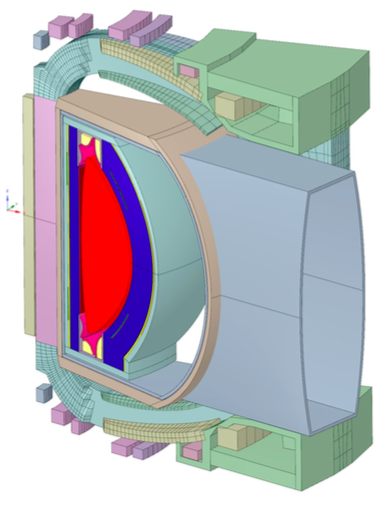
\includegraphics[scale=0.8]{../plots/fess_fnsf_3d_cad.png}
  \caption{The full 3D CAD model of a single FESS-FNSF sector}
  \label{fig:cad_fess_fnsf_3d}
\end{figure}
\section{Analysis Tools}
DAG-MCNP5 coupling
\subsection{Neutron Source Modelling}
Analytic source
\section{Neutron Wall Loading}
Calculations FWs and Divs
\section{Tritium Breeding Calculations}
Introduction
importance of accurate measurements of TBR
\subsection{TBR Workflow}
workflow steps
\subsection{Penetrations and Ports}
figure and results
\subsection{Li-6 Enrichment}
chart
\subsection{TBR mapping}
mapping og NBI, step 7, LH
importance of middle region
\section{Radiation Damage}
\subsection{dpa, He/H production}
at FW and radial distribution of damage
\subsection{Magnet damage}
fast neutron fluence, heating, dpa to Cu stabilizer
\section{Shutdown Dose Rate Calculations}
introduction and r2s worflow
\subsection{SDR}
\subsection{Decay Heat}

\ref{}
\end{document}